\chapter{Generative Adversarial Networks}
\graphicspath{{figs/2de/}}

This exploration delves into the realm of generative models, specifically focusing on Generative Adversarial Networks (GANs) and their conditional variants. GANs have emerged as a groundbreaking concept in unsupervised learning that revolutionized image generation and manipulation. The objective is not only to comprehend the technical mechanisms of GANs but also to recognize their profound impact on image generation, editing, and completion. This exploration also highlights how these models are reshaping our approach to generative tasks within the field of machine learning in a broader context.

\section{Generative Adversarial Networks}

This section presents Generative Adversarial Networks (GANs), a deep learning framework that employs two neural networks, a generator, and a discriminator, in a competitive setup. It offers fundamental insights into how these networks collaborate to produce synthetic data instances that closely resemble real data. The focus is on understanding the architecture, the training procedure, and the core principles, laying the foundation for their various applications in areas such as image generation, style transfer, and beyond.

\subsection{General principles}

\begin{align}
    \min_{G} &\max_{D} \mathbb{E}_{x^* \sim \mathcal{D}\text{ata}} \left[ \log D(x^*) \right] + \mathbb{E}_{z \sim P(z)} \left[ \log (1 - D(G(z))) \right] \label{eq:minimax} \\
    &\max_{G} \mathbb{E}_{z \sim P(z)} \left[ \log D(G(z)) \right] \label{eq:G_maximization} \\
    &\max_{D} \mathbb{E}_{x^* \sim \mathcal{D}\text{ata}} \left[ \log D(x^*) \right] + \mathbb{E}_{z \sim P(z)} \left[ \log (1 - D(G(z))) \right] \label{eq:D_maximization}
\end{align}
    
\paragraph*{1. Interpret the equations \ref{eq:G_maximization} and \ref{eq:D_maximization}. What would happen if we only used one of the two?}

\Cref{eq:G_maximization} describes the goal of the generator $G$ in a GAN. The generator aims to produce images $\tilde{x} = G(z)$ that are indistinguishable from real images by the discriminator. The objective function for the generator maximizes the probability of the discriminator incorrectly classifying these generated images as real. In other words, the generator is trained to "fool" the discriminator. A higher value of $D(G(z))$ implies that the discriminator is more likely to mistake the generated image for a real one, indicating a better performance of the generator.

\Cref{eq:D_maximization} describes the goal of the discriminator $D$ in a GAN. The discriminator's role is to distinguish between real images $x^*$ from the dataset and fake images $\tilde{x}$ produced by the generator. The objective function for the discriminator is to maximize the sum of two terms: the probability of correctly identifying real images as real, and the probability of correctly identifying generated images as fake. The first term $\left(\mathbb{E}_{x^* \sim \mathcal{D}\text{ata}} \left[ \log D(x^*) \right]\right)$ encourages the discriminator to correctly classify real images as real, while the second term $\left(\mathbb{E}_{z \sim P(z)} \left[ \log (1 - D(G(z))) \right]\right)$ pushes it to correctly identify the synthetic images as fake.

If we only used the generator's objective function (\ref{eq:G_maximization}) without the discriminator, the generator would not have a reliable way to measure how good its generated images are. It would lack the feedback mechanism that the discriminator provides, leading to poor-quality image generation. Conversely, if we only used the discriminator's objective function (\ref{eq:D_maximization}) without the generator, the discriminator would only learn to distinguish real images from a static set of fake images. It would not adapt to improving fake images, making it less effective over time as it would not be challenged by increasingly realistic fake images. A GAN relies entirely on the interplay between the generator and discriminator: the generator improves by trying to fool the discriminator, while the discriminator becomes better at distinguishing real from fake images, leading to a dynamic and effective learning process.

\paragraph*{2. Ideally, what should the generator $G$ transform the distribution $P(z)$ to?}

Ideally, the generator $ G $ in a GAN should transform the input noise distribution $ P(z) $ into a distribution that closely resembles the real data distribution $ P(X) $.

In a GAN, $ z $ is a vector sampled from a predefined noise distribution $ P(z) $, which is typically a uniform or normal distribution. The role of the generator $ G $ is to map this noise vector $ z $ into a data point $ \tilde{x} = G(z) $ that appears to have been drawn from the distribution of real data $ P(X) $. The success of the generator is measured by how indistinguishable its output $ \tilde{x} $ is from real data points when evaluated by the discriminator.

The end goal is for the distribution of the generated data $ P_G(X) $ (where $ X $ is generated by $ G(z) $ for $ z \sim P(z) $) to be as close as possible to the real data distribution $ P(X) $. When this happens, the discriminator should find it increasingly difficult to tell apart real data from the generated data, ideally reaching a point where it performs no better than random guessing, resulting in equilibrium, i.e. $\forall x, \, D(x) = 1/2$. This signifies that the generator has effectively learned to produce data that mimics the real data distribution. 

\paragraph*{3. Remark that the equation \ref{eq:G_maximization} is not directly derived from the equation \ref{eq:minimax}. This is justified by the authors to obtain more stable training and avoid the saturation of gradients. What should the ''true'' equation be here?}

In the concept of a GAN, the generator's goal is ideally defined as minimizing the likelihood that the discriminator correctly identifies its outputs as fake. Mathematically, this gives us the following ''true'' equation:

\[
\min_{G} \mathbb{E}_{z \sim P(z)} \left[ \log (1 - D(G(z))) \right]
\]

This objective aims for the generator to produce images that the discriminator will classify as fake (i.e., it tries to minimize the probability of the discriminator being correct). 

\subsection{Architecture of the networks}

\paragraph*{4. Comment on the training of the GAN with the default settings (progress of the generations, the loss, stability, image diversity, etc.).}

In the observed GAN experiments, as training progresses, the generated images increasingly resemble digits. However, the loss values exhibit significant instability, oscillating across epochs, which is a common trait in GAN training, indicating their tendency not to converge in practice. While the generator does improve image quality over time, the generated results still appear noticeably synthetic and limited in diversity, primarily resembling digits such as 0, 3, 7, and 8. This observation raises concerns about a potential mode collapse issue, where the generator learns to produce only a subset of possible outputs that are sufficient to deceive the discriminator but lacks overall diversity.

% j'ai l'impression de pas dire assez => Mettre une image des loss instable et de la faible diversité ? 

\paragraph*{5. Comment on the diverse experiences that you have performed with the suggestions above. In particular, comment on the stability on training, the losses, the diversity of generated images, etc.}

In our experiments, we initially extended the training to 30 epochs. In deep learning, it's a common practice that more epochs can contribute to improved stability, and this was indeed the case in our study. Beyond the 10th epoch, we noticed consistent convergence in subsequent epochs, which resulted in enhanced quality in the generated images.

An intriguing observation was the evolution of the background in these images. Originally black, it gradually developed a form of noise. This change can be attributed to the network's increasing ability to capture and incorporate subtle variations present in the dataset. It indicates the network's growing sophistication in learning complex features. This unexpected transformation in the background texture suggests a more nuanced understanding of the data manifold by the network as the training progressed.

We proceeded to examine the influence of varying the size of the noise vector ($n_z$), a parameter that affects the diversity and complexity of the generated images. Decreasing $n_z$ led to a reduction in diversity among the generated outputs. Conversely, increasing $n_z$ amplified diversity but also introduced complexity to the training process. For these experiments, we kept the number of epochs constant at 5. However, it's noteworthy that, under these conditions, the quality of the generated images was suboptimal when using a large value for $n_z$.

Upon switching to PyTorch's default weight initialization, we observed a delay in the convergence of the GAN, with convergence now occurring around the 11th epoch, compared to the earlier setting. This delay was accompanied by higher error rates throughout the training process. Additionally, the quality of the generated images was notably less convincing when using the default weight initialization compared to the results obtained with the optimized parameters. This outcome highlights the significant impact of customized weight initialization in GANs, as it evidently affects both the training efficiency and the overall quality of the generated images.

% images + mieux commenter les loss ? c'est dur à interpréter PTDR

% the first thought was of course increasing the number of epochs. indeed, in common deep learning problems, increasing number of epochs is synonym of enhanced stability. in our case, it did increase stability, where we see convergence in each of the epochs after reaching the 10th epoch. nit does results in better generated images. one interesting fact is that it also started changing the background, instead of a black background we have some noise?? [why ?]

% then we invesigated the impact of changing $n_z$. Changing the size of the noise vector (nz) affects the variety and complexity of generated images. it is a important parameter. A smaller nz might lead to less diverse outputs, while a larger nz could increase diversity but may also increase training complexity. but here we cannot conclude much, probably bc mnist is a simple dataset ?

% we then changed the weights to use the default ones of pytorch. notably, the gan takes a bit longer to converge 11 epoch and the errors are highers. moreover, the generated images are less convincing that the ones generated using optimized paramers.

% in searching to generate better images, we modified $ngf$ , as Changing the number of generator or discriminator filters can affect the quality and detail of generated images. it lead in a heavier training time. mopreover, the images generated were much clearer. [comment on the losses and errors with the image i provide]

\section{Conditional Generative Adversarial Networks}

This section delves into Conditional Generative Adversarial Networks (cGANs), an advanced variant of GANs. We explore how cGANs extend the GAN framework by introducing conditional variables, enabling more control over the generated outputs. We examine how this added layer of control allows for targeted image generation, enhancing the utility of GANs in tasks like image-to-image translation and targeted style transfer. The focus is on understanding the structural differences from standard GANs and the implications of these changes in practical applications.

\subsection{cDCGAN Architectures for MNIST}

\paragraph*{6. Comment on your experiences with the conditional DCGAN.}

TODO 

% ça marche bien ?

\paragraph*{7. Could we remove the vector $y$ from the input of the discriminator (so having $cD(x)$ instead of $cD(x, y)$)?}

Removing the vector $y$ from the input of the discriminator in a conditional cGAN would significantly alter the network's nature and functionality. The discriminator's role would be reduced to assessing the realism of the images, without the capability to evaluate whether the generated images meet the specified conditions. Consequently, it would be unable to determine whether a generated digit image corresponds to the provided digit label. On the other hand, the generator would still receive $y$ as input. However, with the discriminator no longer enforcing condition compliance, there would be less motivation for the generator to produce images that conform to the specific conditions. This could lead the network towards generating generic, realistic images that may not necessarily align with the intended conditional attributes.

As a result, the model would be proficient at generating realistic images but would lack the capacity to ensure that these images align with specific conditions.

In our experiment, we modified the code to employ an unconditional discriminator while keeping a conditional generator. Our observations supported our hypotheses: because the discriminator lacks conditioning, the generator is not compelled to align with specific conditional inputs. Consequently, the latent space is not effectively conditioned, leading to a lack of consistent correspondence between specific conditions and the generated images. This was evident as the digits appeared to 'move' positions during training, as the discriminator did not impose any particular condition. 

The resulting images in \Cref{fig:cgan_mnist}, although generated, did not conform to the conditional constraints we had defined.  Additionally, we observed mode collapse, where each digit is only associated once, meaning that certain digits were not being adequately represented in the generated samples, leading to a lack of diversity in the output. This underscores the critical role of a conditional discriminator in a cGAN framework, as it ensures that the generated images align with the specified conditions and helps prevent mode collapse by encouraging diversity in the generated samples.

\begin{figure}[H]
    \centering
    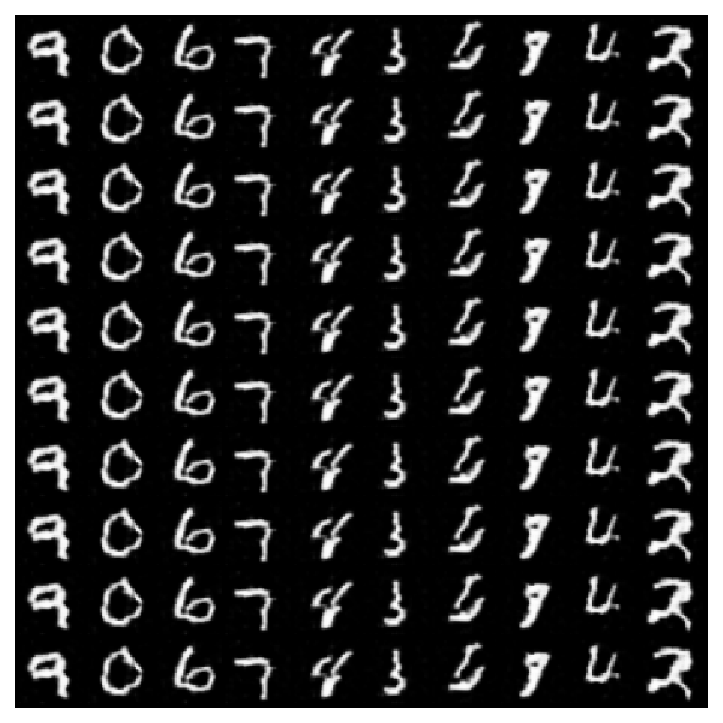
\includegraphics[width=.5\textwidth]{cgan_mnist}
    \caption{Generated digits from a a conditional GAN trained for 10 epochs with the removal of the vector $y$ from the input of the discriminator.}
    \label{fig:cgan_mnist}
\end{figure}

\paragraph*{8. Was your training more or less successful than the unconditional case? Why?}

TODO

% more successful bc thanks to y we now have a gan that produces an image for EACH image, avoiding mode collapse?

\paragraph*{9. Test the code at the end. Each column corresponds to a unique noise vector $z$. What could $z$ be interpreted as here?}

In this context, the noise vector $z$ can be interpreted as the source of randomness or variability that the generator $G$ utilizes to produce different outputs. Each column in \Cref{fig:impact_of_z} corresponds to a unique $z$, and since $z$ is repeated for each class, it serves as a means to generate variations of images across different classes.

Essentially, $z$ acts as a seed for the generative process. Different seeds are expected to yield different images, and with the repetition of $z$ across classes, it's used to generate diverse variations of images corresponding to each class label provided in $y_s$. In summary, $z$ introduces the stochastic element that, in conjunction with class labels, enables the generator to create a variety of images within the specified classes.

\begin{figure}[H]
    \centering
    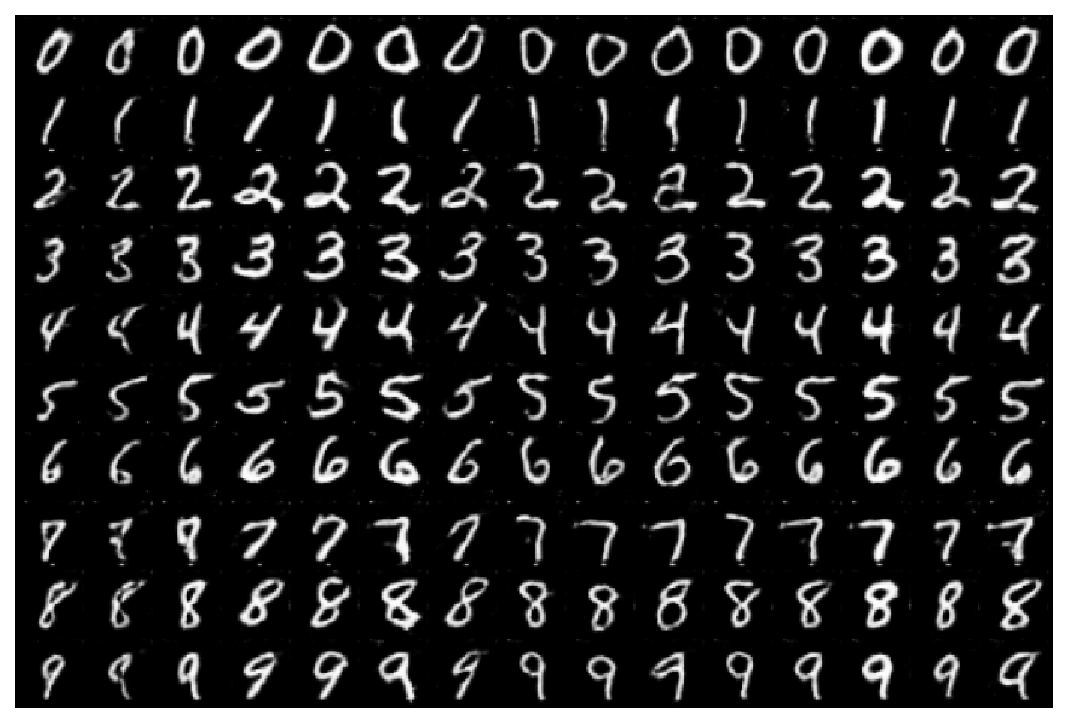
\includegraphics[width=.8\textwidth]{impact_of_z}
    \caption{Influence of a unique noise vector $z$ on our cGAN's generated images.}
    \label{fig:impact_of_z}
\end{figure}